\documentclass[11pt,a4paper,twocolumn]{article}

% ---------------------------------------------------------------
% Layout close to the ACL camera-ready style
% ---------------------------------------------------------------
\usepackage[a4paper,top=2.5cm,bottom=2.5cm,left=2.5cm,right=2.5cm,columnsep=0.6cm]{geometry}
\usepackage[T1]{fontenc}
\usepackage[utf8]{inputenc}
\usepackage{times}
\renewcommand{\ttdefault}{txtt}
\usepackage{latexsym}
\usepackage{amsmath,amssymb}
\usepackage{booktabs}
\usepackage{multirow}
\usepackage{xcolor}
\usepackage{listings}
\usepackage{enumitem}
\usepackage[font=small,labelfont=bf]{caption}
\usepackage{titlesec}
\usepackage{pgfplots}
\pgfplotsset{compat=1.18}
\usepackage[numbers,round,sort&compress]{natbib}
\usepackage[hidelinks]{hyperref}
\usepackage{microtype}
\usepackage{needspace}
\raggedbottom

\titleformat{\section}{\large\bfseries}{\thesection}{1em}{}
\titleformat{\subsection}{\normalsize\bfseries}{\thesubsection}{1em}{}
\titlespacing*{\section}{0pt}{1.2ex plus .3ex}{0.8ex}
\titlespacing*{\subsection}{0pt}{1.0ex plus .3ex}{0.6ex}
\titleformat{\paragraph}[runin]{\normalsize\bfseries}{}{0pt}{}
\titlespacing*{\paragraph}{0pt}{0.9ex plus .3ex}{0.6em}
\setlist{itemsep=2pt,topsep=3pt,parsep=0pt}
\setlength{\textfloatsep}{8pt plus 2pt minus 2pt}
\setlength{\floatsep}{8pt plus 2pt minus 2pt}
\setlength{\dbltextfloatsep}{8pt plus 2pt minus 2pt}
\setlength{\dblfloatsep}{8pt plus 2pt minus 2pt}
\setlength{\abovecaptionskip}{4pt}
\setlength{\belowcaptionskip}{0pt}

\lstset{
  language=Python,
  basicstyle=\ttfamily\small,
  keywordstyle=\bfseries,
  frame=single,
  columns=fullflexible,
  keepspaces=true,
  showstringspaces=false,
  aboveskip=4pt,
  belowskip=0pt
}

\newcommand{\tG}{\tau_G}
\newcommand{\tS}{\tau_S}
\newcommand{\pp}{\,pp}

\definecolor{cG}{RGB}{200,55,45}
\definecolor{cS}{RGB}{35,95,180}
\definecolor{cM}{RGB}{90,90,90}

\title{\Large\bfseries Task Arithmetic with Vision Transformers:\\
An Empirical Analysis of Multi-Task Combination\\
and Task Negation on GTSRB and SVHN}
\author{Luca De Gregorio 2076864\\
Artificial Intelligence and Robotics\\
Sapienza Università di Roma\\
\texttt{degregorio.2076864@studenti.uniroma1.it}}
\date{}

\begin{document}
\maketitle

\begin{center}\textbf{Abstract}\end{center}
\vspace{-0.6ex}
{\small\leftskip=0.6cm\rightskip=0.6cm\noindent
Task arithmetic edits a pre-trained model by adding or subtracting
\emph{task vectors}, the weight differences between fine-tuned and
pre-trained checkpoints. We replicate and extend this framework on two
image-classification tasks, GTSRB and SVHN, with a CLIP ViT-B/16 image
encoder, evaluating 51 edited models in eight experimental phases that
cover scaling, addition, weighted addition and negation. Each task vector
reaches fine-tuned accuracy at $\alpha=1$ (99.2\% on GTSRB, 97.9\% on
SVHN), but neither is task-local: small coefficients transfer positively
to the other task, large ones destroy it, and $\tS$ is markedly more
harmful to GTSRB than $\tG$ is to SVHN. Merging with a shared coefficient
$\alpha=0.5$, which is equivalent to averaging the two fine-tuned models,
retains 97.7\% and 98.5\% of single-task accuracy; independent
coefficients only trade one task against the other along a Pareto front.
Negating a task vector on the base model suppresses the target task but
also removes about 37\pp{} from the other task, whereas negating it in the
presence of the other task's vector is highly selective up to a
coefficient of 0.5 (at most 0.8\pp{} lost on the preserved task) and breaks
down beyond 1.0.\par}

\section{Project Aim and Reference Papers}

This project empirically studies task arithmetic~\citep{ilharco2023}, a
weight-space model-editing framework that composes and suppresses
capabilities of a pre-trained model without any additional training. The
analysis uses a CLIP ViT-B/16 image encoder on two visual classification
benchmarks and is structured around eight progressive experimental phases.
Code and full evaluation logs are available at
\url{https://github.com/2076864/NeuralNetwork}.

\needspace{5\baselineskip}
\paragraph{Reference papers.}
\begin{itemize}
  \item \emph{Editing Models with Task Arithmetic}~\citep{ilharco2023}
  introduces task vectors and shows that adding, negating and combining
  them edits the behaviour of a model in a predictable way.
  \item \emph{Task Singular Vectors: Reducing Task Interference in Model
  Merging}~\citep{gargiulo2025} studies task vectors at the level of
  individual layers. The singular value decomposition of each per-layer
  task matrix shows that these matrices are low-rank and yields a
  layer-wise measure of interference between tasks, which the authors use
  to compress task vectors (TSV-C) and to merge them with reduced
  interference (TSV-M).
\end{itemize}

The central focus of this project is task negation and its interaction
with the other task. \citet{ilharco2023} already use negation to make a
model forget a task, measuring the effect against a control task; here we
complement that analysis by measuring, for a pair of tasks, how negation
behaves with and without an explicit anchor for the task to be preserved.

\section{Introduction: The Case for Task Negation}

Task arithmetic rests on a simple observation: when a model is fine-tuned
on a task, the resulting weight shift encodes that task's knowledge in a
structured, algebraically manipulable form. While multi-task composition
has attracted most of the attention in the model-merging
literature~\citep{ilharco2023,gargiulo2025},
negation has mostly been studied as a forgetting tool evaluated against a
single control task~\citep{ilharco2023}.

Formally, given a pre-trained model $\theta_0$ and a task vector
$\tau_t=\theta_t-\theta_0$, task negation produces
\begin{equation}
  \theta_{\text{neg}} = \theta_0 - \beta\,\tau_t, \qquad \beta>0 .
\end{equation}
If $\tau_t$ encodes the knowledge gained by fine-tuning, then $-\tau_t$
should push the model away from task-specific representations.

\paragraph{Why negation matters.}
\begin{itemize}
  \item \textbf{Unlearning}: removing a specific capability from a deployed
  model without retraining from scratch.
  \item \textbf{Validation of task vector semantics}: if negation reliably
  degrades performance below the zero-shot baseline, the task vector
  encodes task-specific information rather than noise.
  \item \textbf{Selective suppression}: negating one task vector should,
  ideally, affect only the targeted task while leaving the others intact,
  a property we call \emph{selectivity}.
\end{itemize}

\paragraph{Two negation regimes.} We separate two experiments that answer
different questions:
\begin{enumerate}
  \item \textbf{Negation on the base model}, $\theta_0-\beta\,\tau_t$
  (Phase~7): tests whether the task vector is a valid semantic carrier;
  the damage to the other task measures how \emph{non-local} the edit is.
  \item \textbf{Negation in the presence of an anchor},
  $\theta_0+\tau_A-\beta\,\tau_B$ (Phases~5--6; Phase~8 uses the
  equivalent parametrisation $\theta_0+\tau_A+(1-\alpha)\,\tau_B$, i.e.\
  $\beta=\alpha-1$): tests whether negation becomes selective when the
  preserved task is explicitly anchored by its own task vector.
\end{enumerate}

\paragraph{Findings.} (i)~Both task vectors reach fine-tuned accuracy at
$\alpha=1$ and drive their task to chance level or below when negated.
(ii)~Neither vector is task-local: small coefficients help the other task,
large ones destroy it, and $\tS$ harms GTSRB much more than $\tG$ harms
SVHN. (iii)~Weight averaging ($\alpha=0.5$) is a strong merge; independent
coefficients only move along a Pareto front. (iv)~Negation is not
selective on the base model, but becomes highly selective with an anchor,
up to $\beta=0.5$.

\section{Theoretical Background}

\subsection{Task Vectors}
A task vector is the element-wise difference between a fine-tuned model
$\theta_t$ and the shared pre-trained model $\theta_0$:
\begin{equation}
  \tau_t = \theta_t - \theta_0 .
\end{equation}
Applying it with a scaling coefficient $\alpha$ gives
\begin{equation}
  \theta_{\text{new}} = \theta_0 + \alpha\,\tau_t ,
\end{equation}
where $\alpha=0$ recovers the zero-shot model and $\alpha=1$ the
fine-tuned one; $0<\alpha<1$ interpolates between them and $\alpha>1$
extrapolates along the fine-tuning direction.

\subsection{Arithmetic Operations}
\begin{itemize}
  \item \textbf{Scaling} ($\alpha\,\tau_t$) modulates the intensity of the
  learned capability.
  \item \textbf{Addition} ($\tau_A+\tau_B$) combines two tasks in a single
  model, with shared or independent coefficients. With a shared
  $\alpha=0.5$, $\theta_0+0.5(\tau_A+\tau_B)=(\theta_A+\theta_B)/2$:
  simple weight averaging of the two fine-tuned
  models.
  \item \textbf{Negation} ($-\beta\,\tau_t$) suppresses a learned
  capability.
\end{itemize}

\subsection{Interference}
When two task vectors are combined, the loss with respect to the best
single-task model is called interference:
\begin{equation}
  \Delta_t = \mathrm{Acc}_t\!\left(\theta_0+\alpha^*_t\tau_t\right)
           - \mathrm{Acc}_t\!\left(\theta_{\text{merge}}\right),
\end{equation}
where $\alpha^*_t$ is the best single-task coefficient. $\Delta_t>0$
indicates degradation and is expressed in percentage points (pp).
Following~\citet{ilharco2023}, we also report the \emph{normalised
accuracy}
$\mathrm{Acc}_t(\theta_{\text{merge}})/\mathrm{Acc}_t(\theta_0+\alpha^*_t\tau_t)$.

Interference cannot be attributed to non-orthogonality alone:
\citet{ilharco2023} observe that task vectors of different tasks are
typically close to orthogonal. Because the network is non-linear, two
nearly orthogonal weight updates can still interact through shared
activations. \citet{gargiulo2025} argue that a single global similarity
between flattened task vectors is too coarse a description, and measure
interference through the overlap of the singular vectors of each layer;
they also discuss other explanations, such as the redundant parameters and
sign conflicts targeted by TIES-Merging.

\subsection{CLIP ViT-B/16 as Backbone}
The backbone is the image encoder of CLIP, a
Vision Transformer that processes images as
sequences of $16\times16$ patch tokens (12 layers, about 86M parameters)
and was trained contrastively with a text encoder on image--text pairs.
CLIP provides genuine zero-shot classifiers: a class is recognised by
comparing the image embedding with the text embedding of its name.

\section{Implementation Details}

\subsection{Datasets}
\begin{itemize}
  \item \textbf{GTSRB}: 43-class recognition of
  German traffic signs; 12{,}630 test images. Fine-grained classes and
  strong intra-class variability make it a demanding task.
  \item \textbf{SVHN}: 10-class digit recognition
  from street-view house numbers; 26{,}032 test images. Structurally
  simpler, but with background clutter and font variation.
\end{itemize}

\subsection{Models and Checkpoints}
\begin{itemize}
  \item \textbf{Pre-trained checkpoint} (\texttt{zeroshot.pt}): CLIP
  ViT-B/16 image encoder with OpenAI weights, loaded through OpenCLIP,
  used as $\theta_0$ in all experiments.
  \item \textbf{Fine-tuned checkpoints}: the checkpoints released
  with~\citet{ilharco2023} (\texttt{GTSRB/\allowbreak finetuned.pt} and
  \texttt{SVHN/\allowbreak finetuned.pt}), obtained by fine-tuning the
  image encoder from $\theta_0$ with the classification head frozen.
  \item \textbf{Classification heads} (\texttt{head\_GTSRB.pt},
  \texttt{head\_SVHN.pt}): zero-shot heads built by encoding the class
  names with the CLIP text encoder and dataset-specific prompt templates.
  They stay fixed throughout, so task vectors only concern the image
  encoder; they cover all its floating-point parameters.
\end{itemize}

\subsection{Experimental Setup}
All models are evaluated in \texttt{eval} mode on the full test sets, and
top-1 accuracy is reported. Evaluations ran on a consumer laptop with a
2\,GB NVIDIA GPU; the edited encoder occupies about 0.46\,GB of GPU memory. Phases~0--6 used a batch
size of 32 and Phases~7--8 a batch size of 128; since the ViT uses only
per-sample normalisation, predictions do not depend on the batch size,
which Phase~8 confirms (Section~\ref{sec:phase8}).

For accuracies above 90\%, the binomial standard error is below 0.3\pp{}
on GTSRB and 0.2\pp{} on SVHN, so differences of a few tenths of a point
should not be over-interpreted. All coefficients were selected directly
on the test sets (Section~\ref{sec:limits}).

The original \texttt{TaskVector} class supports addition and negation but
not multiplication by a scalar, so a small helper scales the parameter
dictionary directly (Listing~\ref{lst:scaletv}).

\begin{lstlisting}[float=t,caption={Helper used to scale a task vector by an arbitrary (also negative) coefficient.},label={lst:scaletv}]
def scale_tv(tv, alpha):
    scaled = copy.deepcopy(tv)
    scaled.vector = {
        k: v * alpha
        for k, v in tv.vector.items()
    }
    return scaled
\end{lstlisting}

\subsection{Eight-Phase Protocol}
Table~\ref{tab:protocol} lists the phases. Phases~1--3 sweep
$\alpha\in\{-0.5,0,0.5,1,1.5,2\}$ (negative values coincide with
Phase~7 and are not repeated in the tables), Phase~4 tests ten
coefficient pairs, Phases~5--6 use $\beta\in\{0.3,0.5,0.7,1.0,1.5\}$ and
Phases~7--8 use $\{0.5,1.0,1.5\}$. In total, 51 models are evaluated on
both datasets.

\begin{table}[t]
\centering\small
\begin{tabular}{@{}cll@{}}
\toprule
Phase & Name & Formula \\
\midrule
0 & Zero-shot baseline & $\theta_0$ \\
1 & Solo $\tG$ & $\theta_0+\alpha\,\tG$ \\
2 & Solo $\tS$ & $\theta_0+\alpha\,\tS$ \\
3 & Shared $\alpha$ & $\theta_0+\alpha(\tG+\tS)$ \\
4 & Independent $\alpha$'s & $\theta_0+\alpha_1\tG+\alpha_2\tS$ \\
5 & Anchored neg.\ of $\tG$ & $\theta_0+\tS-\beta\,\tG$ \\
6 & Anchored neg.\ of $\tS$ & $\theta_0+\tG-\beta\,\tS$ \\
7 & Neg.\ on base model & $\theta_0-\beta\,\tau_t$ \\
8 & Neg.\ on multi-task & $\theta_0+\tau_A+(1-\alpha)\,\tau_B$ \\
\bottomrule
\end{tabular}
\caption{Overview of the eight experimental phases. Phase~8 is a
reparametrisation of Phases~5--6 with $\beta=\alpha-1$.}
\label{tab:protocol}
\end{table}

\section{Results and Analysis}

\subsection{Phase 0 --- Zero-Shot Baseline}

\begin{table}[t]
\centering\small
\begin{tabular}{@{}lrr@{}}
\toprule
Model & GTSRB & SVHN \\
\midrule
CLIP ViT-B/16 zero-shot & 43.3\% & 52.0\% \\
\bottomrule
\end{tabular}
\caption{Phase 0: zero-shot baseline.}
\label{tab:phase0}
\end{table}

These values (Table~\ref{tab:phase0}) are the reference point for all
other phases: results below them indicate active suppression or
inadvertent degradation.

\subsection{Phases 1 \& 2 --- Single Task Vectors}

\begin{table}[t]
\centering\small
\begin{tabular}{@{}llrr@{}}
\toprule
Phase & $\alpha$ & GTSRB & SVHN \\
\midrule
\multirow{4}{*}{1 --- $\tG$}
 & $+0.5$ & 97.9\% & 59.9\% \\
 & $+1.0$ & \textbf{99.2\%} & 55.9\% \\
 & $+1.5$ & 98.6\% & 29.7\% \\
 & $+2.0$ & 94.1\% & 13.3\% \\
\midrule
\multirow{4}{*}{2 --- $\tS$}
 & $+0.5$ & 47.2\% & 97.0\% \\
 & $+1.0$ & 28.7\% & \textbf{97.9\%} \\
 & $+1.5$ & 14.2\% & 97.2\% \\
 & $+2.0$ & 5.1\% & 95.7\% \\
\bottomrule
\end{tabular}
\caption{Phases 1 \& 2: single task vector sweep. Each vector also
changes the accuracy on the other task (zero-shot: 43.3\% GTSRB, 52.0\%
SVHN).}
\label{tab:phase12}
\end{table}

Both task vectors reach their best accuracy at the fine-tuned point,
$\alpha^*_G=\alpha^*_S=1.0$ (Table~\ref{tab:phase12}, Figure~\ref{fig:sweep}).
Over-scaling degrades the target task only mildly (94.1\% on GTSRB and
95.7\% on SVHN at $\alpha=2$).

\paragraph{Cross-task effects.} Neither vector leaves the other task
unchanged, and the effect is not monotonic. A small dose transfers
positively: $0.5\,\tG$ raises SVHN from 52.0\% to 59.9\% (+7.9\pp) and
$0.5\,\tS$ raises GTSRB from 43.3\% to 47.2\% (+3.9\pp). Larger doses are
destructive: at $\alpha=2$ SVHN falls to 13.3\% and GTSRB to 5.1\%. The
two directions are asymmetric already at $\alpha=1$, i.e.\ for the
fine-tuned models themselves: fine-tuning on GTSRB still improves SVHN
(+3.9\pp), whereas fine-tuning on SVHN reduces GTSRB by 14.6\pp, well
below its zero-shot level. This asymmetry recurs in every later phase.

\begin{figure*}[t]
\centering
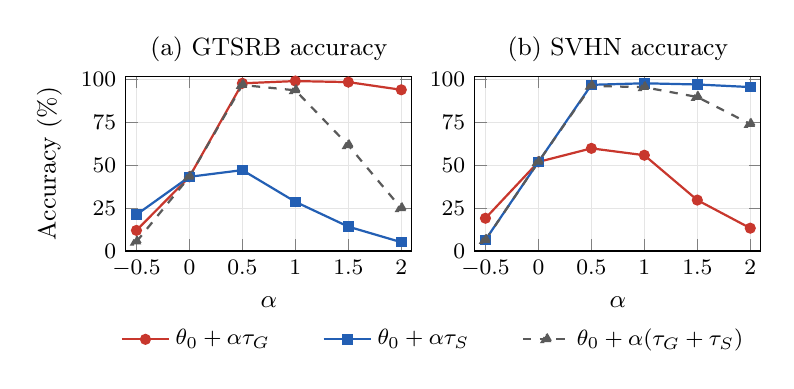
\begin{tikzpicture}
\begin{axis}[
  name=left, width=0.43\textwidth, height=3.8cm,
  title={\small (a) GTSRB accuracy}, title style={yshift=-1ex},
  xlabel={\small $\alpha$}, ylabel={\small Accuracy (\%)},
  xmin=-0.6, xmax=2.1, ymin=0, ymax=102,
  xtick={-0.5,0,0.5,1,1.5,2}, ytick={0,25,50,75,100},
  tick label style={font=\footnotesize},
  grid=major, grid style={gray!20},
  legend style={font=\footnotesize, at={(1.08,-0.38)}, anchor=north, draw=none, legend columns=3, /tikz/every even column/.append style={column sep=0.6cm}},
  legend cell align=left]
\addplot[cG, thick, mark=*, mark size=1.6pt] coordinates {(-0.5,12.0)(0,43.3)(0.5,97.9)(1,99.2)(1.5,98.6)(2,94.1)};
\addlegendentry{$\theta_0+\alpha\tau_G$}
\addplot[cS, thick, mark=square*, mark size=1.5pt] coordinates {(-0.5,21.2)(0,43.3)(0.5,47.2)(1,28.7)(1.5,14.2)(2,5.1)};
\addlegendentry{$\theta_0+\alpha\tau_S$}
\addplot[cM, thick, dashed, mark=triangle*, mark size=2pt] coordinates {(-0.5,5.4)(0,43.3)(0.5,96.9)(1,93.8)(1.5,61.7)(2,24.9)};
\addlegendentry{$\theta_0+\alpha(\tau_G+\tau_S)$}
\end{axis}
\begin{axis}[
  at={(left.east)}, anchor=west, xshift=0.8cm,
  width=0.43\textwidth, height=3.8cm,
  title={\small (b) SVHN accuracy}, title style={yshift=-1ex},
  xlabel={\small $\alpha$},
  xmin=-0.6, xmax=2.1, ymin=0, ymax=102,
  xtick={-0.5,0,0.5,1,1.5,2}, ytick={0,25,50,75,100},
  tick label style={font=\footnotesize},
  grid=major, grid style={gray!20}]
\addplot[cG, thick, mark=*, mark size=1.6pt] coordinates {(-0.5,19.1)(0,52.0)(0.5,59.9)(1,55.9)(1.5,29.7)(2,13.3)};
\addplot[cS, thick, mark=square*, mark size=1.5pt] coordinates {(-0.5,6.5)(0,52.0)(0.5,97.0)(1,97.9)(1.5,97.2)(2,95.7)};
\addplot[cM, thick, dashed, mark=triangle*, mark size=2pt] coordinates {(-0.5,6.4)(0,52.0)(0.5,96.4)(1,95.6)(1.5,89.9)(2,74.1)};
\end{axis}
\end{tikzpicture}
\caption{Scaling sweeps of Phases 1--3 (the points at $\alpha=-0.5$
coincide with Phase~7 at $\beta=0.5$). Each task vector helps the other
task at small $\alpha$ and destroys it at large $\alpha$; in the merged
model, GTSRB collapses much faster than SVHN for $\alpha>1$.}
\label{fig:sweep}
\end{figure*}

\subsection{Phase 3 --- Multi-Task Combination}

\begin{table}[t]
\centering\small
\begin{tabular}{@{}lrr@{}}
\toprule
$\alpha$ & GTSRB & SVHN \\
\midrule
$0.0$ & 43.3\% & 52.0\% \\
$+0.5$ & \textbf{96.9\%} & \textbf{96.4\%} \\
$+1.0$ & 93.8\% & 95.6\% \\
$+1.5$ & 61.7\% & 89.9\% \\
$+2.0$ & 24.9\% & 74.1\% \\
\bottomrule
\end{tabular}
\caption{Phase 3: shared-$\alpha$ multi-task combination.}
\label{tab:phase3}
\end{table}

The best shared coefficient is $\alpha=0.5$, i.e.\ the average of the two
fine-tuned models, with 96.9\% on GTSRB and 96.4\% on SVHN
(Table~\ref{tab:phase3}). With respect to the single-task upper bounds,
\begin{align*}
\Delta_G &= 99.2-96.9 = 2.3\,\text{pp},\\
\Delta_S &= 97.9-96.4 = 1.5\,\text{pp},
\end{align*}
corresponding to normalised accuracies of 97.7\% and 98.5\%. Most of this
gap comes from halving each vector rather than from the other vector: at
$\alpha=0.5$ the single-task models reach 97.9\% and 97.0\%, so adding the
second half-vector costs only 1.0\pp{} on GTSRB and 0.6\pp{} on SVHN.

The plain sum ($\alpha=1$) is clearly worse (93.8\% and 95.6\%, i.e.\
$\Delta_G=5.4$\pp, $\Delta_S=2.3$\pp), and for $\alpha>1$ GTSRB collapses
much faster than SVHN (24.9\% vs.\ 74.1\% at $\alpha=2$). GTSRB is the more
fragile task in the merged model, consistent with the strong damage that
$\tS$ alone causes on GTSRB in Phase~2.

\subsection{Phase 4 --- Independent Coefficients}

\begin{table}[t]
\centering\small
\begin{tabular}{@{}lrrr@{}}
\toprule
$(\alpha_1,\alpha_2)$ & GTSRB & SVHN & Avg \\
\midrule
$(0.3, 0.3)$ & 88.8\% & 91.0\% & 89.9\% \\
$(0.5, 0.3)$ & 97.8\% & 90.1\% & 94.0\% \\
$(0.3, 0.5)$ & 86.1\% & 97.0\% & 91.6\% \\
$(0.5, 0.5)^\dagger$ & 96.9\% & 96.4\% & 96.7\% \\
$(0.6, 0.4)$ & 98.4\% & 93.9\% & 96.2\% \\
$(0.4, 0.6)$ & 91.4\% & \textbf{97.4\%} & 94.4\% \\
$(0.7, 0.5)^\dagger$ & 98.5\% & 95.3\% & \textbf{96.9\%} \\
$(0.5, 0.7)^\dagger$ & 93.7\% & \textbf{97.4\%} & 95.6\% \\
$(0.8, 0.5)^\dagger$ & \textbf{98.8\%} & 94.4\% & 96.6\% \\
$(0.5, 0.8)$ & 90.0\% & \textbf{97.4\%} & 93.7\% \\
\bottomrule
\end{tabular}
\caption{Phase 4: weighted combination $\alpha_1\tG+\alpha_2\tS$.
$^\dagger$Pareto-optimal among the tested pairs. The $(0.5,0.5)$ row
reproduces Phase~3 exactly.}
\label{tab:phase4}
\end{table}

No pair improves both tasks with respect to $(0.5,0.5)$
(Table~\ref{tab:phase4}): independent coefficients move the model along a
Pareto front formed by $(0.5,0.7)$, $(0.5,0.5)$, $(0.7,0.5)$ and
$(0.8,0.5)$. All other pairs are dominated; for instance, $(0.4,0.6)$ has
the same SVHN accuracy as $(0.5,0.7)$ but 2.3\pp{} less on GTSRB.

The front is shaped by the same asymmetry observed above. Raising
$\alpha_2$ from 0.5 to 0.8 gains 1.0\pp{} on SVHN but costs 6.9\pp{} on
GTSRB, whereas raising $\alpha_1$ from 0.5 to 0.8 gains 1.9\pp{} on GTSRB
and costs only 2.0\pp{} on SVHN: the marginal damage of $\tS$ on GTSRB is
about 3.5 times that of $\tG$ on SVHN. Giving $\tG$ the larger weight is
therefore the better trade-off, and $(0.7,0.5)$ achieves the highest
average (96.9\%), raising GTSRB by 1.6\pp{} at the cost of 1.1\pp{} on
SVHN. Its advantage over $(0.5,0.5)$ (0.2\pp{} on average) is, however,
of the same order as the sampling error.

\subsection{Phases 5 \& 6 --- Anchored Negation}

\begin{table}[t]
\centering\small
\begin{tabular}{@{}llrrr@{}}
\toprule
Phase & $\beta$ & GTSRB & SVHN & $\Delta_A$ \\
\midrule
\multirow{5}{*}{\shortstack[l]{5\\$\tS-\beta\tG$}}
 & 0.3 & 15.2\% & 97.6\% & $-0.3$ \\
 & 0.5 & 9.8\% & 97.1\% & $-0.8$ \\
 & 0.7 & 5.6\% & 96.3\% & $-1.6$ \\
 & 1.0 & 3.0\% & 93.5\% & $-4.4$ \\
 & 1.5 & 2.7\% & 64.8\% & $-33.1$ \\
\midrule
\multirow{5}{*}{\shortstack[l]{6\\$\tG-\beta\tS$}}
 & 0.3 & 98.9\% & 23.4\% & $-0.3$ \\
 & 0.5 & 98.4\% & 11.1\% & $-0.8$ \\
 & 0.7 & 96.5\% & 7.2\% & $-2.7$ \\
 & 1.0 & 75.6\% & 6.4\% & $-23.6$ \\
 & 1.5 & 11.9\% & 6.5\% & $-87.3$ \\
\bottomrule
\end{tabular}
\caption{Phases 5 \& 6: negation in the presence of an anchor.
$\Delta_A$: change (pp) of the anchored task with respect to its
single-task model (97.9\% SVHN in Phase~5, 99.2\% GTSRB in Phase~6).}
\label{tab:phase56}
\end{table}

Phases~5 and~6 negate one task vector while keeping the other one at full
strength (Table~\ref{tab:phase56}, Figure~\ref{fig:negation}). For
moderate coefficients negation is highly selective: up to $\beta=0.5$ the
anchored task loses at most 0.8\pp, while the target task is pushed far
below its value in the anchored model (GTSRB from 28.7\% to 9.8\%, SVHN
from 55.9\% to 11.1\%).

Selectivity breaks down for larger coefficients, and again
asymmetrically. With the SVHN anchor, SVHN loses 4.4\pp{} at $\beta=1$ and
33.1\pp{} at $\beta=1.5$; with the GTSRB anchor, GTSRB already loses
23.6\pp{} at $\beta=1$ and collapses to 11.9\% at $\beta=1.5$. Together with
Phases~2--4, this indicates that large perturbations along $\pm\tS$ are
especially damaging for GTSRB.

\begin{figure*}[t]
\centering
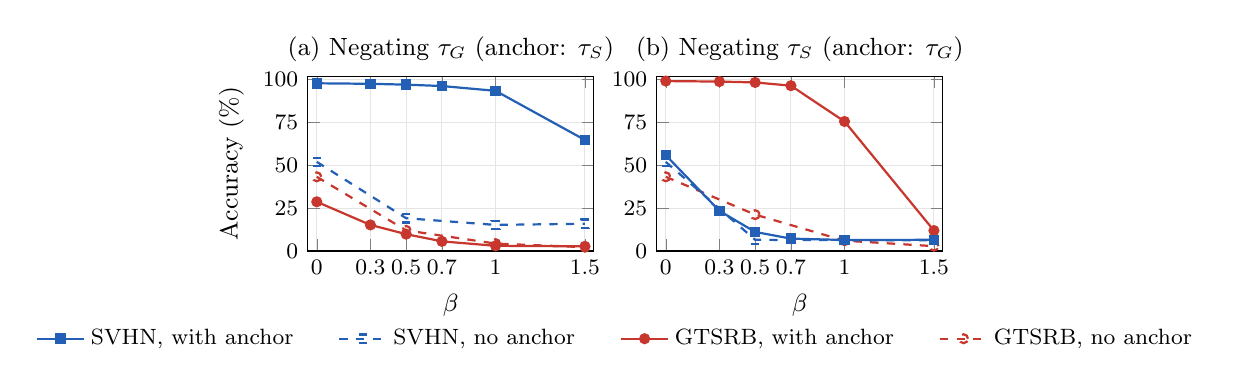
\begin{tikzpicture}
\begin{axis}[
  name=left, width=0.43\textwidth, height=3.8cm,
  title={\small (a) Negating $\tau_G$ (anchor: $\tau_S$)}, title style={yshift=-1ex},
  xlabel={\small $\beta$}, ylabel={\small Accuracy (\%)},
  xmin=-0.05, xmax=1.55, ymin=0, ymax=102,
  xtick={0,0.3,0.5,0.7,1,1.5}, ytick={0,25,50,75,100},
  tick label style={font=\footnotesize},
  grid=major, grid style={gray!20},
  legend style={font=\footnotesize, at={(1.08,-0.38)}, anchor=north, draw=none, legend columns=4, /tikz/every even column/.append style={column sep=0.5cm}},
  legend cell align=left]
\addplot[cS, thick, mark=square*, mark size=1.5pt] coordinates {(0,97.9)(0.3,97.6)(0.5,97.1)(0.7,96.3)(1.0,93.5)(1.5,64.8)};
\addlegendentry{SVHN, with anchor}
\addplot[cS, thick, dashed, mark=square, mark size=1.5pt] coordinates {(0,52.0)(0.5,19.1)(1.0,15.2)(1.5,15.9)};
\addlegendentry{SVHN, no anchor}
\addplot[cG, thick, mark=*, mark size=1.6pt] coordinates {(0,28.7)(0.3,15.2)(0.5,9.8)(0.7,5.6)(1.0,3.0)(1.5,2.7)};
\addlegendentry{GTSRB, with anchor}
\addplot[cG, thick, dashed, mark=o, mark size=1.6pt] coordinates {(0,43.3)(0.5,12.0)(1.0,4.3)(1.5,2.2)};
\addlegendentry{GTSRB, no anchor}
\end{axis}
\begin{axis}[
  at={(left.east)}, anchor=west, xshift=0.8cm,
  width=0.43\textwidth, height=3.8cm,
  title={\small (b) Negating $\tau_S$ (anchor: $\tau_G$)}, title style={yshift=-1ex},
  xlabel={\small $\beta$},
  xmin=-0.05, xmax=1.55, ymin=0, ymax=102,
  xtick={0,0.3,0.5,0.7,1,1.5}, ytick={0,25,50,75,100},
  tick label style={font=\footnotesize},
  grid=major, grid style={gray!20}]
\addplot[cG, thick, mark=*, mark size=1.6pt] coordinates {(0,99.2)(0.3,98.9)(0.5,98.4)(0.7,96.5)(1.0,75.6)(1.5,11.9)};
\addplot[cG, thick, dashed, mark=o, mark size=1.6pt] coordinates {(0,43.3)(0.5,21.2)(1.0,6.0)(1.5,2.8)};
\addplot[cS, thick, mark=square*, mark size=1.5pt] coordinates {(0,55.9)(0.3,23.4)(0.5,11.1)(0.7,7.2)(1.0,6.4)(1.5,6.5)};
\addplot[cS, thick, dashed, mark=square, mark size=1.5pt] coordinates {(0,52.0)(0.5,6.5)(1.0,6.3)(1.5,6.3)};
\end{axis}
\end{tikzpicture}
\caption{Negation with and without an anchor. Solid lines:
$\theta_0+\tau_A-\beta\,\tau_B$ (Phases 5, 6 and 8); dashed lines:
$\theta_0-\beta\,\tau_B$ (Phase 7). Without an anchor the preserved task
collapses together with the target; with an anchor it stays within
0.8\pp{} of its single-task accuracy up to $\beta=0.5$.}
\label{fig:negation}
\end{figure*}

\subsection{Phase 7 --- Negation on the Base Model}

\begin{table}[t]
\centering\small
\begin{tabular}{@{}llrr@{}}
\toprule
Sub-phase & $\beta$ & GTSRB & SVHN \\
\midrule
\multirow{3}{*}{7a --- $-\beta\,\tG$}
 & 0.5 & 12.0\% & 19.1\% \\
 & 1.0 & 4.3\% & 15.2\% \\
 & 1.5 & 2.2\% & 15.9\% \\
\midrule
\multirow{3}{*}{7b --- $-\beta\,\tS$}
 & 0.5 & 21.2\% & 6.5\% \\
 & 1.0 & 6.0\% & 6.3\% \\
 & 1.5 & 2.8\% & 6.3\% \\
\bottomrule
\end{tabular}
\caption{Phase 7: negation on the base model. Zero-shot: 43.3\% GTSRB,
52.0\% SVHN; chance level: 2.3\% GTSRB, 10\% SVHN.}
\label{tab:phase7}
\end{table}

Both task vectors are valid semantic carriers (Table~\ref{tab:phase7}):
negating $\tG$ brings GTSRB from 43.3\% to 2.2\%, close to chance
($1/43\approx2.3\%$), and negating $\tS$ brings SVHN from 52.0\% to 6.3\%.
Beyond $\beta\approx1$ the target accuracy no longer decreases. For SVHN
the plateau lies well \emph{below} chance (10\%), which indicates
systematic rather than random errors; a plausible explanation is that the
model collapses onto one or a few classes, since a constant prediction of
a single minority digit would score in this range on the imbalanced SVHN
test set.

\paragraph{Collateral damage.} On the base model negation is not
selective: at $\beta=1$, negating $\tG$ also removes 36.8\pp{} from SVHN
(52.0\%$\rightarrow$15.2\%) and negating $\tS$ removes 37.3\pp{} from GTSRB
(43.3\%$\rightarrow$6.0\%). This is consistent with representations shared
by the two tasks, but it does not by itself prove that $\tG$ and $\tS$
overlap: in a non-linear network, a large perturbation in almost any
direction can degrade all tasks. The comparison with Phases~5--6 isolates
the role of the anchor: the same $-0.5\,\tG$ costs SVHN 32.9\pp{} on the
base model but only 0.8\pp{} when $\tS$ is present
(Figure~\ref{fig:negation}).

\subsection{Phase 8 --- Negation on the Multi-Task Model}
\label{sec:phase8}

\begin{table}[t]
\centering\small
\begin{tabular}{@{}llrr@{}}
\toprule
Sub-phase & $\alpha$ & GTSRB & SVHN \\
\midrule
\multirow{3}{*}{\shortstack[l]{8a\\$\tS+(1-\alpha)\tG$}}
 & 0.5 & 75.8\% & 97.5\% \\
 & 1.0 & 28.7\% & \textbf{97.9\%} \\
 & 1.5 & 9.8\% & 97.1\% \\
\midrule
\multirow{3}{*}{\shortstack[l]{8b\\$\tG+(1-\alpha)\tS$}}
 & 0.5 & \textbf{99.0\%} & 91.2\% \\
 & 1.0 & \textbf{99.2\%} & 55.9\% \\
 & 1.5 & 98.4\% & 11.1\% \\
\bottomrule
\end{tabular}
\caption{Phase 8: negation on the multi-task model. $\alpha=1.0$
reproduces Phases~2 and~1 exactly; $\alpha=1.5$ coincides with
Phases~5 and~6 at $\beta=0.5$.}
\label{tab:phase8}
\end{table}

\paragraph{Sanity check.} Phase~8 evaluates
$\theta_0+\tau_A+(1-\alpha)\,\tau_B$ (Table~\ref{tab:phase8}), which at
$\alpha=1$ reduces to $\theta_0+\tau_A$. Phase~8a reproduces Phase~2 to the second decimal on
both datasets (28.65\% GTSRB, 97.86\% SVHN) and Phase~8b reproduces
Phase~1 (99.17\% GTSRB, 55.87\% SVHN). The two phases were run with
different batch sizes (32 and 128), so the match also confirms that the
evaluation is deterministic and batch-independent.

\paragraph{Relation to Phases 5--6.} Since
$\theta_0+\tau_A+(1-\alpha)\tau_B=\theta_0+\tau_A-(\alpha-1)\tau_B$, only
$\alpha>1$ corresponds to negation, and $\alpha=1.5$ is the same model as
Phases~5--6 at $\beta=0.5$; the results are indeed identical (9.8\%/97.1\%
and 98.4\%/11.1\%). At $\alpha=0.5$ the vector $\tau_B$ is \emph{added}
with weight 0.5, which extends the Phase~4 grid to $(1.0,0.5)$ (99.0\%
GTSRB, 91.2\% SVHN) and $(0.5,1.0)$ (75.8\%, 97.5\%). Phase~8 is therefore
a consistency check rather than an independent experiment: the
selectivity evidence comes from Phases~5--6.

\section{Conclusions}

\begin{itemize}
  \item \textbf{Task vectors are valid and reproducible carriers.} Each
  reaches fine-tuned accuracy at $\alpha=1$, and negating it drives its
  task to chance level or below. Independent runs of the same model
  agree to the second decimal.
  \item \textbf{Task vectors are not task-local.} A small dose of one
  vector improves the other task, a large dose destroys it. The effect is
  asymmetric: $\tS$ harms GTSRB much more than $\tG$ harms SVHN, and this
  asymmetry shapes every combination we tested.
  \item \textbf{Weight averaging is a strong merge.} With $\alpha=0.5$ the
  merged model keeps 97.7\% (GTSRB) and 98.5\% (SVHN) of single-task
  accuracy. Independent coefficients do not improve both tasks; they move
  along a Pareto front, on which giving more weight to $\tG$, e.g.\
  $(0.7,0.5)$, is the better trade-off.
  \item \textbf{Negation needs an anchor.} On the base model, negation
  also removes about 37\pp{} from the other task. With the other task's
  vector present, it is highly selective up to $\beta=0.5$ but fails
  beyond $\beta=1$, earlier when GTSRB is the task to preserve.
\end{itemize}

In practice, both merging and unlearning by task arithmetic require a
careful calibration of the coefficients: moderate values ($\alpha\approx
0.5$ for merging, $\beta\le0.5$ for anchored negation) give the best
balance between the tasks.

\section{Limitations and Future Work}
\label{sec:limits}

\paragraph{Computational constraints.} The 51 models required 102
evaluation passes of about 34 minutes (GTSRB) and 70 minutes (SVHN) each,
roughly 88 hours on a 2\,GB laptop GPU. This limited both the number of
tasks and the density of the coefficient grids.

\paragraph{Two-task scope.} With only GTSRB and SVHN we cannot tell
whether the observed asymmetry and the selectivity of anchored negation
generalise; the reference papers~\citep{ilharco2023,gargiulo2025} use
8 or more tasks.

\paragraph{Coefficient selection on the test set.} All coefficients were
chosen on the test sets, without a separate validation split, so the
reported optima are slightly optimistic. Differences of a few tenths of a
point, such as $(0.7,0.5)$ vs.\ $(0.5,0.5)$, are within sampling error.

\paragraph{Missing geometric analysis.} We did not measure the norms of
$\tG$ and $\tS$, their cosine similarity, or the per-layer interference
of their singular vectors~\citep{gargiulo2025}, which could explain why
$\tS$ is more harmful to GTSRB than the converse.

\paragraph{Baselines for negation.} A random vector with the same
per-layer norm as $\tau_t$~\citep{ilharco2023} would separate task-specific
suppression from generic damage caused by a large perturbation, and a
confusion matrix of the negated SVHN model would test the class-collapse
hypothesis.

\paragraph{Merging methods.} More advanced methods, such as TSV-Merge or
the other merging techniques compared by \citet{gargiulo2025}, might shift
the Pareto front observed in Phase~4.

\small\raggedright
\setlength{\bibsep}{2pt}
\begin{thebibliography}{2}

\bibitem[Ilharco et~al.(2023)]{ilharco2023}
Editing Models with Task Arithmetic.
\newblock \emph{International Conference on Learning Representations (ICLR)}, 2023.\\
\url{https://arxiv.org/abs/2212.04089}

\bibitem[Gargiulo et~al.(2025)]{gargiulo2025}
A Survey on Model Merging in the Era of Large Language Models.
\newblock \emph{arXiv preprint arXiv:2412.00081}, 2024.\\
\url{https://arxiv.org/abs/2412.00081}

\end{thebibliography}

\end{document}
